\chapter{Background} \label{chap:background}

% Boustrophedon cell decomposition based coverage method 
% not Boustrophedon area coverage from right to left and from left to right in alternate lines.
% veer the uav from the desired path

The merit of this thesis in the coverage path planning context is splitting and decoupling the process of the coverage problem. The process will consist of: finding the proper pose and orientation of camera views that maintain area coverage, then apply path planning techniques to traverse these poses. So that the first part can be used as a solution by itself with positioning cameras in the obtained positions. The second merit is minimizing the overlapping paths and implementing the path planning taking into account the footprint of the robot and the camera, not relying on the assumption of robot representation as a point. % here the footprint of the camera only not the robot too 

\section{Related Work in path planning}
\subsection{Coverage Path Planning}
There are two main surveys that this literature review is relying on in picking and comparing the path planning technique to be further implemented and tested on the quadcopter. These surveys are; a survey on coverage path planning for robotics \cite{CPP2} and coverage for robotics survey of recent results\cite{CPP1}. 
% Also the books like latombe , principle of mobile robot 
There are a lot of other work extensively explored from many research areas beside path planning like computer vision and graph theory. The problem can be studied from many sides like mapping, searching, patrolling, and applications. We focus here on the path planning and area coverage problems with slightly different approach than the common one. we take into consideration the footprint of the camera and one of the goals is to reduce the number of waypoints with maximum area coverage. Full area coverage in terms of 100\% is not the constraint.

In the literature generally there is always a navigation pattern to pass through the whole space; the robot needs to cover. This pattern is done after decomposing the map into either regular cells or irregular ones like Voronoi. These methods can be categorized as heuristic and approximate, partial-approximate and exact cellular decompositions as discussed in \cite{CPP1}.

%Coverage algorithms can be classified as heuristic or complete depending on whether or not they provably guarantee complete coverage of the free space. At the same time, they can be classified as online or offline. Offline algorithms rely only on the stationary information, and the environment is assumed to be known. Usually online algorithms are needed if some kind of adaptivity to the environment is required. Online algorithms usually utilize real-time sensor measurements. Thus, these algorithms can also be called sensor-based coverage algorithms.
Coverage algorithms can be classified as heuristic or complete depending on whether or not they provably guarantee complete coverage of the free space. They can also be classified as online or offline based on when they are going to be applied. In the case of being applied to the robot while it is executing its path, then it is online. They are considered offline if a prior map is given and the path planning is obtained, and then the robot execute this path.
 
The heuristic approach that is based on a random path which is like the one equipped in some lawn mower and vacuum cleaner robots as mentioned in \cite{CPP1}. This approach can not be considered for aerial robots applications due to its expensive time and energy costs.

Coverage algorithms can rely on cellular decomposition with many techniques that an extensive comparison was given in \cite{CPP2}. Then an ox plowing motions (Boustrophedon manner) is used like the example in planning algorithm book \cite{planningBook}. As the approach used in this thesis will not rely on map decomposition, further investigation can be found in the cited papers and book.

%\textcolor{red}{ If not decomposition how to say grid decomposition } 


%\textcolor{red}{These algorithm can result in redundant coverage.}

Other approaches like  Artificial Potential Fields (APF), node based (graph) algorithms and neural networks can be used instead of the map decomposition. %\textcolor{red}{||||||}




\subsection{Coverage Path Planning for UAVs}
There are various ways to obtain and optimize the path planning. CPP problem is a sub-field of path planning and well studied for ground vehicles like cases in \cite{CPP1,CPP2,path_planning_UGV}.

%\textbf{CPP for UAV in general} 

In operations research, the CPP problem represents the environment as a graph. The problem can be represented as the travelling salesman problem(TSP) or postman problems to generate optimal solutions. In the graph representation, locations in the environment is represented as nodes in the graph and the paths between the locations are the edges. Each edge has a cost assigned to it. The cost can represent measurements such as distance(Euclidean,Mahalanobis,etc) between locations, terrain traversability, travel time or a combination of several metrics. These edges can be constrained or unconstrained with directions. More precisely undirected , directed graphs.

Voronoi diagram is also another possible solution as developed in \cite{voronoi_UAV} for decomposing the desired area and find the feasible solution from the starting point to the goal point through two-step path planning algorithm, but it doesn't take into consideration the repetition rate constraint or full area coverage. For these reasons considering problem representation as arc routing problem is most beneficial. Solving these problems can be achieved by using bio-inspired algorithms like neural networks or evolutionary algorithms.

TSP is considered one problem of a large class of problems known as combinatorial problems. It is introduced in UAV path planning for several purposes like refueling depots in \cite{TSP_UAV}, multiple UAV cooperative reconnaissance in \cite{TSP_UAV_Multi}. This is a non-deterministic polynomial-time hard (NP-hard) problem, that is sub-optimally solvable by many approaches as found in various research fields \cite{TSP_NPHARD}. Evolutionary approaches specifically will be considered in this thesis.  
% \cite{papadimitriou1977euclidean}

\subsubsection*{Evolutionary algorithms}

% \textbf{In this thesis considering one UAV operation to solve the CPP problem using GA as global path planning followed by local path planning solution.} 

Evolutionary Algorithms(EA) as a sub branch of meta-heuristic optimization algorithms, imitates the biological process of evolution in nature. There are various algorithms that are branched from it like Ant colony optimization (ACO), particle swarm optimization (PSO),Genetic Algorithm GA and much more which can be studied from \cite{Evo_Book1,Evo_Book2}. GA uses techniques of inheritances, mutations, selections and crossovers of chromosomes over several generations of possible solutions to find convergence to the most optimized solution. Explanation in the next chart is the general abstract view of GA, more details will be explained in the methodology chapters.

\tikzset{
  frame/.style={
    rectangle, draw, 
    text width=6em, text centered,
    minimum height=4em,drop shadow,fill=lime!40,
    rounded corners,
  },
  line/.style={
    draw, -latex',rounded corners=3mm,
  }
}

\begin{tikzpicture}[font=\small\sffamily\bfseries,very thick,node distance = 4cm]
\node [frame] (pop) {Population};
\node [above=2cm, left of=pop] (init) {Initialisation};
\node [below=2cm, left of=pop] (term) {Termination};
\node [frame, above=2cm, right of=pop] (parents)  {Parents};
\node [frame, below=2cm, right of=pop] (off)  {Offspring};

\path [line] (parents)
 -- node[right,align=left,pos=.5] {Cross-Over\\[3mm]Mutation}
 (off);
\path [line] (init) |- (pop.170);
\path [line] (pop.190) -| (term);
%tournament 
\path [line] (off) -| node[below,pos=.25, align=center] {Survivor\\ selection}(pop);
\path [line] (pop) |- node[above,pos=.75, align=center] {Parents\\ selection}(parents);

% \circledarrow{ultra thick, gray}{text}{1cm};

\end{tikzpicture}

Coverage path planning can be categorized into sampling based algorithms, node based algorithms, mathematic model based algorithms, bio-inspired algorithms. Then comes the category emerging lately in the next subsection.

\subsection{Hybrid Algorithms for path planning}

%\textbf{A two-level approach to collision-free navigation, using
%artificial potential fields on the local lower solution planning, and GA solution to waypoints optimization problem represented as TSP for global higher layer planning}. 
%
%then point-to-point motion planning problem, where the vehicle task is to navigate from a pre-specified initial point in the workspace to a pre-specified destination goal point.
Having hybrid path planning algorithms by combining several algorithms together to achieve better performance. These combinations comes in terms of fusing several path planning algorithms in a layer by layer way. This will lead to better solutions to overcome the problems like local minima, long time to find the solution, sharp-edged paths. The algorithms fusion can be simultaneous or successive. For instance, Scholer et all \cite{scholer2012generating} applied visibility graph, then Dijkstra’s algorithm to find an optimal solution for UAV path planning problem in 3D.

%Xiao et all [6] used 3D grid to represent the environment and 3D PRM to form a roadmap in obstacle
%free space, at last A* optimal search algorithm combined to achieve an optimal path. Masehian et all[56]
%introduced a visibility graph, Voronoi diagram, and potential field(VVP) integrated algorithm. If investigate
%the extension of VVP algorithm to 3D space, it shows effective tradeoff between the shortest and safest path.
%Scholer et all[115] combined visibility graph and Dijkstra’s algorithm( or Geodesics ) to find an optimal
%solution for path planning problem in 3D. Jaishankar [116] planned outdoor environment path by citing
%GIS-MCDA approach which first synthesizes a various of information to generate a ’combined gray level
%image’, then an optimal searching algorithm as A*, or D*, or EA is used to achieve an optimal path. A
%hybrid of mathematic model based algorithms with EA [117] is proposed to solve to solve NP-hard problem,
%where general EA tend to be premature. A lot of works adopt this idea, this paper gives a pioneering work
%of coming up with a taxonomy of this kind of methods.

\section{Waypoints Selection}

Finding the waypoints to have the best coverage of the area is close to the problem of positioning cameras or sensors to cover an area efficiently. Sensor positioning problem has been investigated since a few decades, mainly for video surveillance \cite{c1}. Without any additional constraint, this problem is NP-Hard as stated in \cite{c1,c2,c3,c4,c5} for the Watchman Route Problem (which is very similar to the optimal positioning waypoint for UAV path). Two non-optimal solutions have been proposed. The first one is based on Art Gallery Problem (AGP) \cite{c2,c3} and the second one is based on the Wireless Sensors Networks \cite{c6,c7,c8,c9} trying to find the best position to design an efficient network which can collect data with any kind of sensors. 

% do you mean here the the sensor pose is the most adequate solution

However, the solution proposed to the problem addressed the coverage problem but linked with additional and specific constraints, which are out of our scope. 
% like basic room without obstacles or focus on selection among the different possible sensor poses, which is the most adequate solutions. 
% This will become finding a solution among a set of more efficient subset of solutions, not a problem of finding a solution
%This will not become a problem of finding a position but to select among the set of more efficient subset of solutions. %or select the position sensor in the set of possible and restrained position
 %\cite{c7}.
 
 One of the algorithms used is the Particle Swarm Optimization (PSO) as detailed in \cite{c10,c11}. Zhou \textit{et al.} \cite{c10}, some experimental results are provided and one solution running in real time is proposed. However, the scene used in these experiments is rather small and many cameras are employed to fully cover it.  On the other hand, \cite{c11} uses a cost function but the cost function is not only focused on the position for surveillance and coverage, but also handling resolution and lighting, which affect the final solution by not covering the under illuminated areas.Reddy \textit{et al}. \cite{c11} also introduced the concept of an “acceptable response”, allowing non-optimal/sub-optimal solutions. If the coverage score is higher than a given threshold, the solution is accepted and not locked by the research of an optimal solution. 
% Inspired by \cite{c10,c11}, extending the method for UAV waypoints positioning and path planning in more complex environments (basic room, big room, non-square shape).
 
 \section{UAV Localization} \label{localization_Back}
 
UAV localization problem is the challenge of finding the pose in terms of position and orientation of the aerial robot from the reference frame. This reference frame can be the initial point the robot is launched from, or a point on the map. There are two main categories for localizing the robot; either indoor or outdoor. For outdoor, GPS-based navigation system is often used to determine the UAV’s absolute position. Also equipped with inertial measurement unit (IMU), UAV's orientation and acceleration can be estimated. State estimation of the UAV is obtained by coupling the previously obtained data with the UAV's or/and environment mathematical model. This information is essential for autonomous navigation and of significant importance to aid the pilot to achieve smoother navigation.

 Unlike ground vehicles, just holding the robot's pose requires motor orders to withstand and hover its place, giving order continuously to the robot. This is particularly the case for an aerial vehicle - while for ground-based vehicles not moving typically is a trivial task. Holding a position in the air requires constantly counteracting minor randomly induced movements, which in turn requires a method to detect these movements.
While for indoor localization challenge; GPS data can not be reliable. Also employing the IMU data can provide relative location, over time small errors will keep accumulating and drift will happen and affect the localization. Additional information about global positioning should be available to recover for this drift using means of filtering and sensor fusion \cite{benini2013imu}. 

These alternative localization methods can be categorized as     
\begin{itemize}
\item Rely only on the UAV's sensors IMU, onboard camera.
\item External fiducial markers tracked by onboard camera.
\item Using external tracking devices.
\end{itemize}

\begin{figure}[!h]
  \centering
  \subfigure[AR tags]{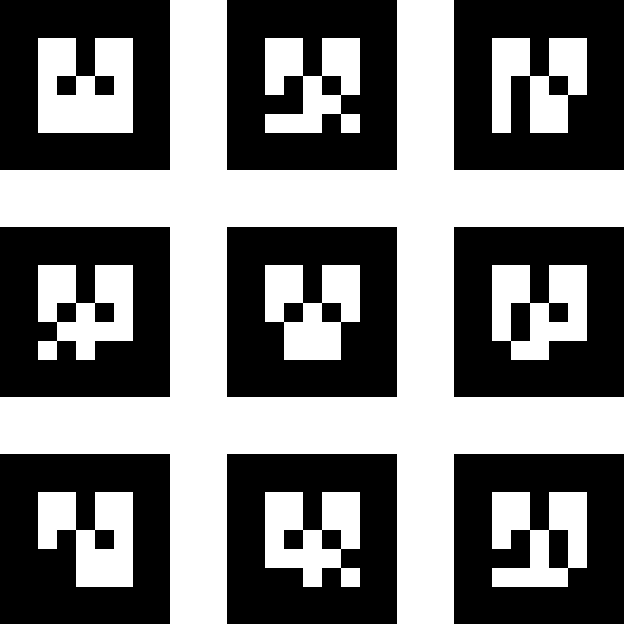
\includegraphics[width=0.4\textwidth]{figures/markers0to8.png}}
  \hfill
  \subfigure[Motion tracking cameras]{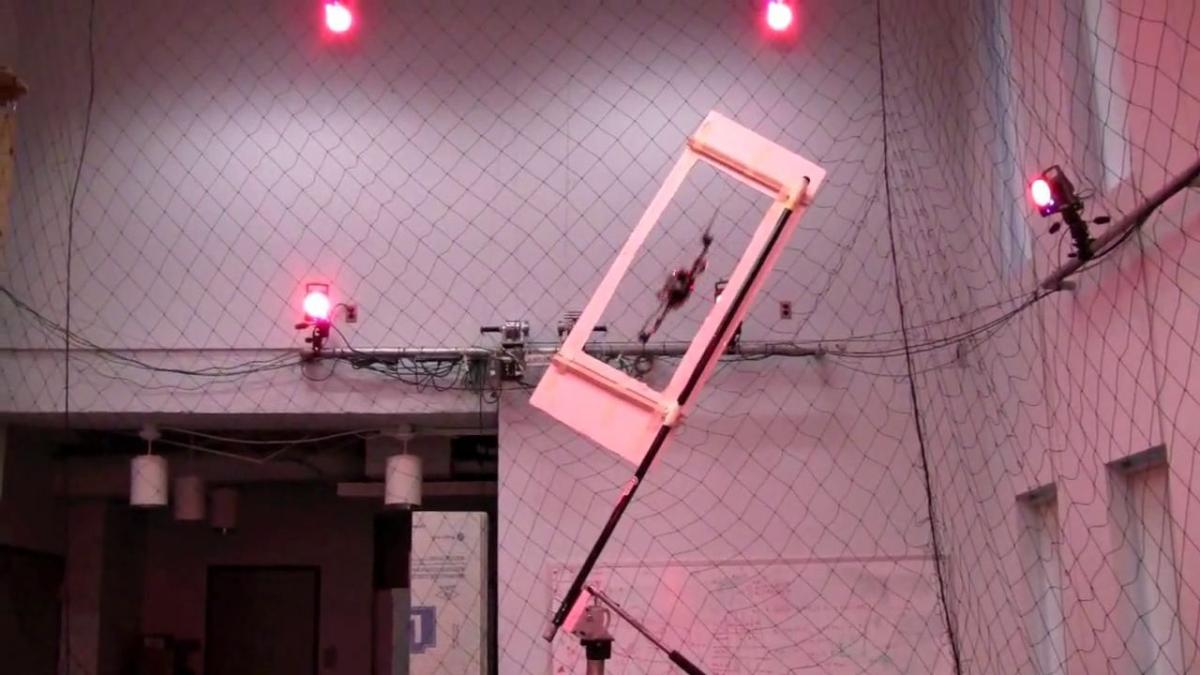
\includegraphics[width=0.55\textwidth]{figures/quadrotor_vicon_motion_capture_2.jpg}}
  \caption{Localization techniques}
  \label{fig:final_room}
\end{figure}

An example of the available external tracking device is motion capture camera that allow the robot to measure its position with very high precision and accuracy as in \cite{michael2010grasp}. Reflective markers like retroreflective dots attached to the robot, the cameras can estimate the position of each reflective marker and these cameras can do it at split second timing exceeding speeds of 100-200 times a second. This system will not be used as it requires setup up of several cameras which cost dozens of thousands of euros. The other external solution provided for example in  \cite{meier2012pixhawk} using external markers and detected using onboard camera. This solution could have been considered, but it is not the chosen one to be implemented in this thesis. 
 
 
 There is wide range of sensors can be equipped on the UAV to help its localization like laser range scanner, monocular camera, stereo camera, RGB-D sensor, or ultrasonic range sensors. The usage of the monocular camera is chosen to be the solution for this thesis. They provide competitive advantages; as they are cheap, energy-efficient, small and light. For instance, the system of navigation in this paper \cite{fei2013comprehensive} is based on vision optical flow and laser FastSLAM.
 
 Simultaneous localization and mapping (SLAM) can be achieved by combining visual pose estimates from the monocular camera  with additional sensor measurements available like the implementation of Tardif et al. in \cite{tardif2008monocular}. The tool developed by the computer vision group at the Technical University of Munich as mentioned in the papers \cite{engel14ras,engel12iros}, is utilized on an AR.Drone 2.0 available in the lab with minor modification. 
 
\section{Mosaicking}
%Mosaicing is one of the techniques of image processing which is useful for tiling digital images. Mosaicing is blending together of several arbitrarily shaped images to form one large radiometrically balanced image so that the boundaries between the original images are not seen. Any number of geocoded images can be blended together along user-specified cut lines (polygons). Mosaicing is a special case of geometric correction where registration takes place in the existing image. If ground control points (GCP) are collected the input image is transformed according to the derived polynomial into the output image. If no GCPs are provided, but both images already have compatible georeferencing, then an appropriate translation and scaling will be applied instead of polynomial transformation. This technique is generally used on several images like remote sensed images, bio-medical images or other digital images. This paper attempts to develop a package for mosaicing multiple images. The work has been divided into three modules. Each module is run independently. These modules are (1) Images are displayed in overview, full resolution/zoomed modes, (2) Registration and layout file generation, (3) Polygon filling, blending and displaying of mosaiced images. These modules can be integrated to form a full-fledged system
Mosaicking is one of the active research areas in computer vision field. It is a technique used to blend several images together to form a larger image. The images captured by the UAV during flight are pieced together to construct a mosaicked image from overlapping photographs. 

% http://www.imageprocessingplace.com/downloads_V3/root_downloads/tutorials/An_Introduction_to_Image_Mosaicing.htm

The problem of mosaicking can be solved by addressing three main problems:

\begin{itemize}
\item Correct geometrical deformations
\item Image registration
\item Eliminate seams from image mosaics
\end{itemize}

Image registration can be emphasised in research by finding the point-to-point correspondence in different views of the same scene. Plane surface under general camera motion can be related by planar projective transformation, called homography. The homography matrix is 3x3 8 degree of freedom (DOF). This can ensure mosaicking of images captured by the camera rotating around its field of projection in \cite{zheng1992panoramic}.

% \cite{suzuki2010vision} for uav image mosaicing
More details about introductory information can be found in \cite{mosaic_image_intro,capel2004image} .

%without considering the features of the images, but relying on the given position and orientation. 
 
%  feature based : http://cseweb.ucsd.edu/classes/fa02/cse252c/smallick.pdf

%  comparison : http://citeseerx.ist.psu.edu/viewdoc/download?doi=10.1.1.677.1527&rep=rep1&type=pdf